%%%%%%%%%%%%%%%%%%%%%%%%%%%%%%%%%%%%%%%%%
% Short Sectioned Assignment
% LaTeX Template
% Version 1.0 (5/5/12)
%
% This template has been downloaded from:
% http://www.LaTeXTemplates.com
%
% Original author:
% Frits Wenneker (http://www.howtotex.com)
%
% License:
% CC BY-NC-SA 3.0 (http://creativecommons.org/licenses/by-nc-sa/3.0/)
%
%%%%%%%%%%%%%%%%%%%%%%%%%%%%%%%%%%%%%%%%%

%----------------------------------------------------------------------------------------
%	PACKAGES AND OTHER DOCUMENT CONFIGURATIONS
%----------------------------------------------------------------------------------------

\documentclass[paper=a4, fontsize=11pt]{scrartcl} % A4 paper and 11pt font size

\usepackage[T1]{fontenc} % Use 8-bit encoding that has 256 glyphs
\usepackage{fourier} % Use the Adobe Utopia font for the document - comment this line to return to the LaTeX default
\usepackage[english]{babel} % English language/hyphenation
\usepackage{amsmath,amsfonts,amsthm,mathtools,amssymb} % Math packages
\usepackage{dsfont} %double stroke
\usepackage[margin=1.75cm]{geometry}
\usepackage{multicol}
\usepackage{setspace}
\usepackage{graphicx}
\usepackage{setspace}
\onehalfspacing
\usepackage{multicol}
\allowdisplaybreaks
\usepackage{hyperref}

% R code
\usepackage{listings}

    \lstset{
    language=R,
    basicstyle=\scriptsize\ttfamily,
    commentstyle=\ttfamily\color{gray},
    numbers=left,
    numberstyle=\ttfamily\color{gray}\footnotesize,
    stepnumber=1,
    numbersep=5pt,
    backgroundcolor=\color{white},
    showspaces=false,
    showstringspaces=false,
    showtabs=false,
    frame=single,
    tabsize=2,
    captionpos=b,
    breaklines=true,
    breakatwhitespace=false,
    title=\lstname,
    escapeinside={},
    keywordstyle={},
    morekeywords={}
    }
% Binomial tree
\usepackage{tikz}
\usetikzlibrary{matrix}

% Permutations and combinations 
\newcommand*{\Perm}[2]{{}^{#1}\!P_{#2}}%
\newcommand*{\Comb}[2]{{}^{#1}C_{#2}}%

\usepackage{sectsty} % Allows customizing section commands
\allsectionsfont{\raggedright \normalfont} % Make all sections left, the default font and small caps
\renewcommand{\thesubsection}{\alph{subsection}} % Make the subsections letters
\newcommand{\rreduce}[2]{\mathop{\longrightarrow}_{\tiny{#1}}}

\usepackage{float} % picture placement
\usepackage{subfig} % picture placement
\usepackage{fancyhdr} % Custom headers and footers
\pagestyle{fancyplain} % Makes all pages in the document conform to the custom headers and footers
\fancyhead{} % No page header - if you want one, create it in the same way as the footers below
\fancyfoot[L]{} % Empty left footer
\fancyfoot[C]{} % Empty center footer
\fancyfoot[R]{\thepage} % Page numbering for right footer
\renewcommand{\headrulewidth}{0pt} % Remove header underlines
\renewcommand{\footrulewidth}{0pt} % Remove footer underlines
\setlength{\headheight}{13.6pt} % Customize the height of the header

\numberwithin{equation}{section} % Number equations within sections (i.e. 1.1, 1.2, 2.1, 2.2 instead of 1, 2, 3, 4)
\numberwithin{figure}{section} % Number figures within sections (i.e. 1.1, 1.2, 2.1, 2.2 instead of 1, 2, 3, 4)
\numberwithin{table}{section} % Number tables within sections (i.e. 1.1, 1.2, 2.1, 2.2 instead of 1, 2, 3, 4)

\setlength\parindent{0pt} % Removes all indentation from paragraphs - comment this line for an assignment with lots of text

%----------------------------------------------------------------------------------------
%	TITLE SECTION
%----------------------------------------------------------------------------------------

\newcommand{\horrule}[1]{\rule{\linewidth}{#1}} % Create horizontal rule command with 1 argument of height

\title{	
\normalfont \normalsize 
\textsc{University of Chicago | Financial Mathematics} \\ [25pt] % Your university, school and/or department name(s)
\horrule{0.5pt} \\[0.4cm] % Thin top horizontal rule
\huge FINM 33150: Homework 1 \\ % The assignment title
\horrule{2pt} \\[0.5cm] % Thick bottom horizontal rule
}

\author{Michael Beven - 455613} % Your name

\date{\normalsize\today} % Today's date or a custom date

\begin{document}

\maketitle % Print the title

%----------------------------------------------------------------------------------------
%	PROBLEM 3
%----------------------------------------------------------------------------------------

\section*{3.}

First we load modules:

\begin{verbatim}
# load key packages
library(MASS)
library(Quandl)
library(ggplot2)
library(stringr)
library(R.cache)
library(plotly)
\end{verbatim}

Then we add memoization and load the data:

\begin{verbatim}
# add memoization
reload.data <- TRUE
QLoad <- R.cache::addMemoization(Quandl::Quandl)

# load data
if (reload.data == TRUE) {
  Quandl.api_key('v21snmSix9KyXBWc1RkF')
  cat('Data Reload/n')
  msft.raw <- QLoad('YAHOO/MSFT')
  bac.raw <- QLoad('WIKI/BAC')
}
\end{verbatim}

Next we set the data to a 'birth month' and then clean the data:

\begin{verbatim}
# take desired dates
msft <- subset(msft.raw, msft.raw$Date >= as.Date('1990-10-15') & 
                 msft.raw$Date <= as.Date('1990-11-09'))
bac <- subset(bac.raw, bac.raw$Date >= as.Date('1990-10-15') & 
                bac.raw$Date <= as.Date('1990-11-09'))

# add index code to data, so we don't confuse them
names(msft) <- paste('YAHOO.MSFT -',names(msft))
names(bac) <- paste('WIKI.BAC -',names(bac))
# fix renamed date column
names(msft)[1] <- 'Date'
names(bac)[1] <- 'Date'
# merge data
df <- merge(msft,bac)

# function to clean Quandl names
clean.quandl.name <- function(x) {
  cleaned <- x
  if (x=='Date') {
    
  } else {
    tryCatch({
      parts <- stringr::str_split(x, " - ",n=2)
      first.parts <- stringr::str_split(parts[[1]][[1]], "\\.",n=2)
      cleaned <- paste(first.parts[[1]][[2]], parts[[1]][[2]], sep=".")
      cleaned <- str_replace_all(cleaned," ","")
    },
    error = function(e) {cat(paste0("Err on",x,"\n"))}
    )
  }
  stringr::str_trim(cleaned)
}

# use clean.quandl.name
fixed.names <- lapply(names(df),clean.quandl.name)
cat(paste(fixed.names,sep="\n"))
df.renamed <- df
names(df.renamed) <- fixed.names
\end{verbatim}

We only need a subset of the data, which is the close prices:

\begin{verbatim}
# only need close data
df.renamed.close <- subset(df.renamed, select=c('MSFT.Close','BAC.Close'))
\end{verbatim}

Now, we can run a linear regression on the close prices:

\begin{verbatim}
# linear regression on close prices of MSFT vs. BAC
regress <- lm(df.renamed.close$MSFT.Close ~ df.renamed.close$BAC.Close)
print(summary(regress))

Call:
lm(formula = df.renamed.close$MSFT.Close ~ df.renamed.close$BAC.Close)

Residuals:
    Min      1Q  Median      3Q     Max 
-6.8500 -1.0604  0.6566  2.0960  3.7273 

Coefficients:
                           Estimate Std. Error t value Pr(>|t|)    
(Intercept)                 76.6265     9.5847   7.995 2.47e-07 ***
df.renamed.close$BAC.Close  -0.7174     0.4907  -1.462    0.161    
---
Signif. codes:  0 '***' 0.001 '**' 0.01 '*' 0.05 '.' 0.1 ' ' 1

Residual standard error: 3.041 on 18 degrees of freedom
Multiple R-squared:  0.1061,	Adjusted R-squared:  0.05647 
F-statistic: 2.137 on 1 and 18 DF,  p-value: 0.161
\end{verbatim}

then, we create log returns from the data subset and run a regression on that:

\begin{verbatim}
# create log returns data
N <- dim(df.renamed.close)[1]
df.logrets <- log(df.renamed.close[2:N,]) - log(df.renamed.close[1:N-1,])
regress.logrets <- lm(df.logrets$MSFT.Close ~ df.logrets$BAC.Close)
print(summary(regress.logrets))

Call:
lm(formula = df.logrets$MSFT.Close ~ df.logrets$BAC.Close)

Residuals:
      Min        1Q    Median        3Q       Max 
-0.041179 -0.015816 -0.004455  0.013457  0.069918 

Coefficients:
                      Estimate Std. Error t value Pr(>|t|)
(Intercept)           0.007217   0.006040   1.195    0.249
df.logrets$BAC.Close -0.035116   0.172365  -0.204    0.841

Residual standard error: 0.02631 on 17 degrees of freedom
Multiple R-squared:  0.002436,	Adjusted R-squared:  -0.05624 
F-statistic: 0.04151 on 1 and 17 DF,  p-value: 0.841
\end{verbatim}

Finally, plot:

\begin{verbatim}
# plot of regression of prices
pdf('RegPrices.pdf')
plot(df.renamed.close$BAC.Close,df.renamed.close$MSFT.Close,pch=20,ylim=c(45,60),
     xlim=c(15,20),xlab='BAC.Close',ylab='MSFT.Close',
     main='Regression of Microsoft Close Price Against Bank of America Close Price')
abline(regress)
dev.off()

# plot of regression of returns
pdf('RegRets.pdf')
plot(df.logrets$BAC.Close,df.logrets$MSFT.Close,pch=20,xlab='BAC.Close',
     ylab='MSFT.Close',ylim=c(-0.02,0.1),xlim=c(-0.02,0.1),
     main='Regression of Microsoft Close Return Against Bank of America Close Return')
abline(regress.logrets)
dev.off()
\end{verbatim}

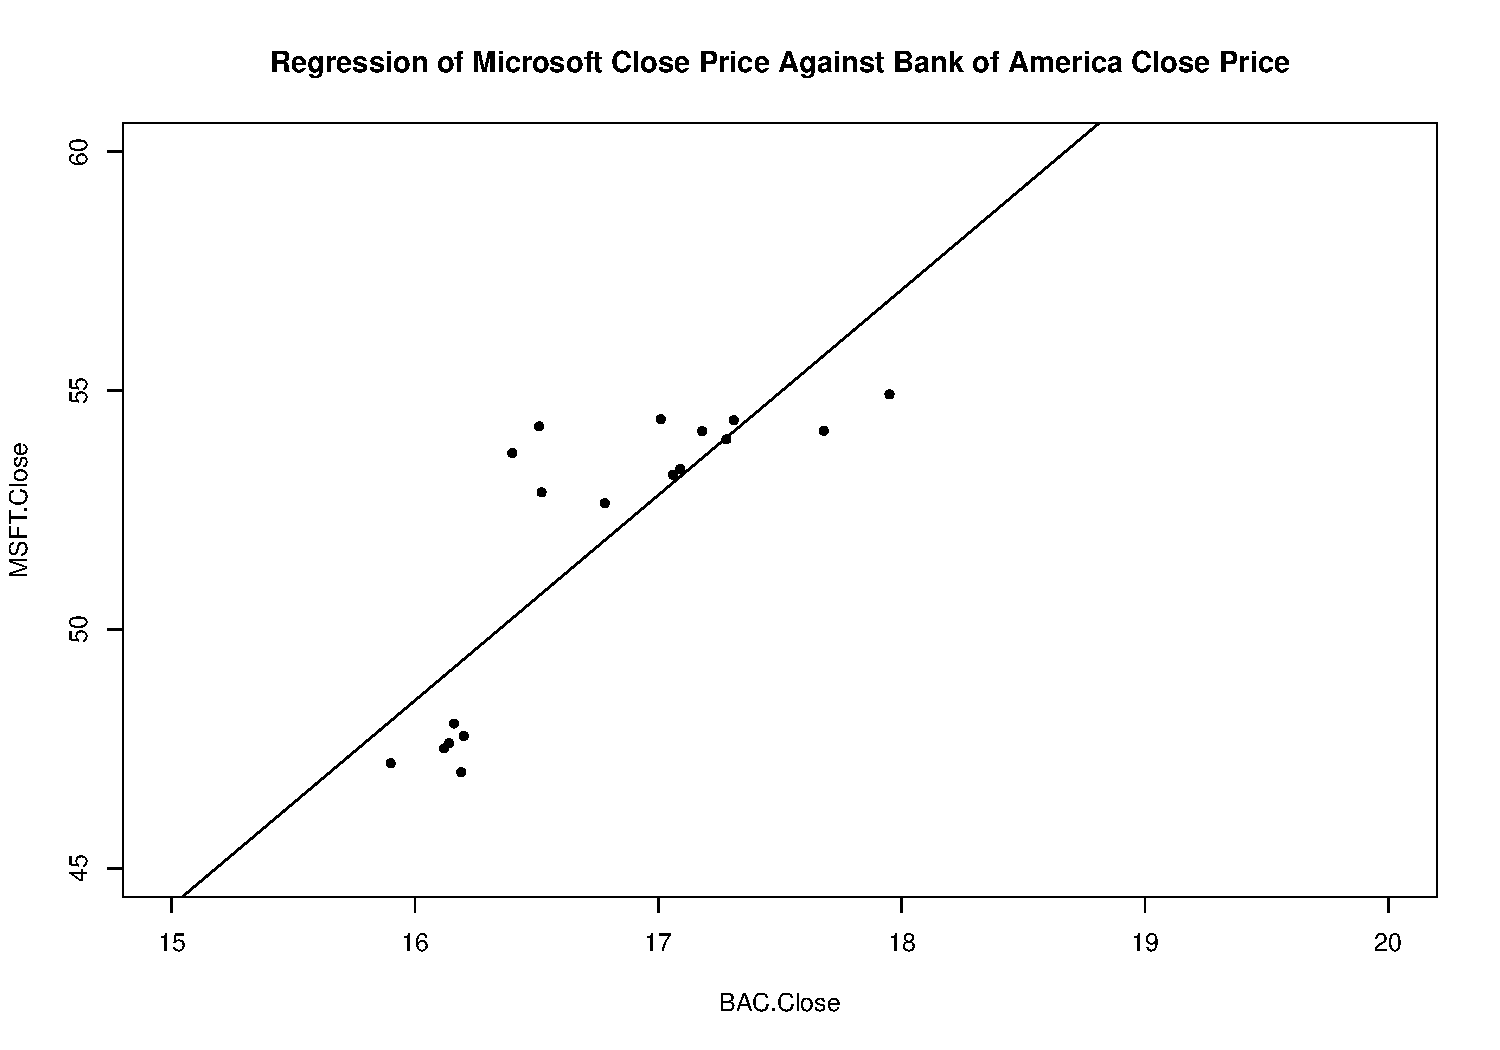
\includegraphics[scale=0.6]{RegPrices.pdf}\centering

\raggedright

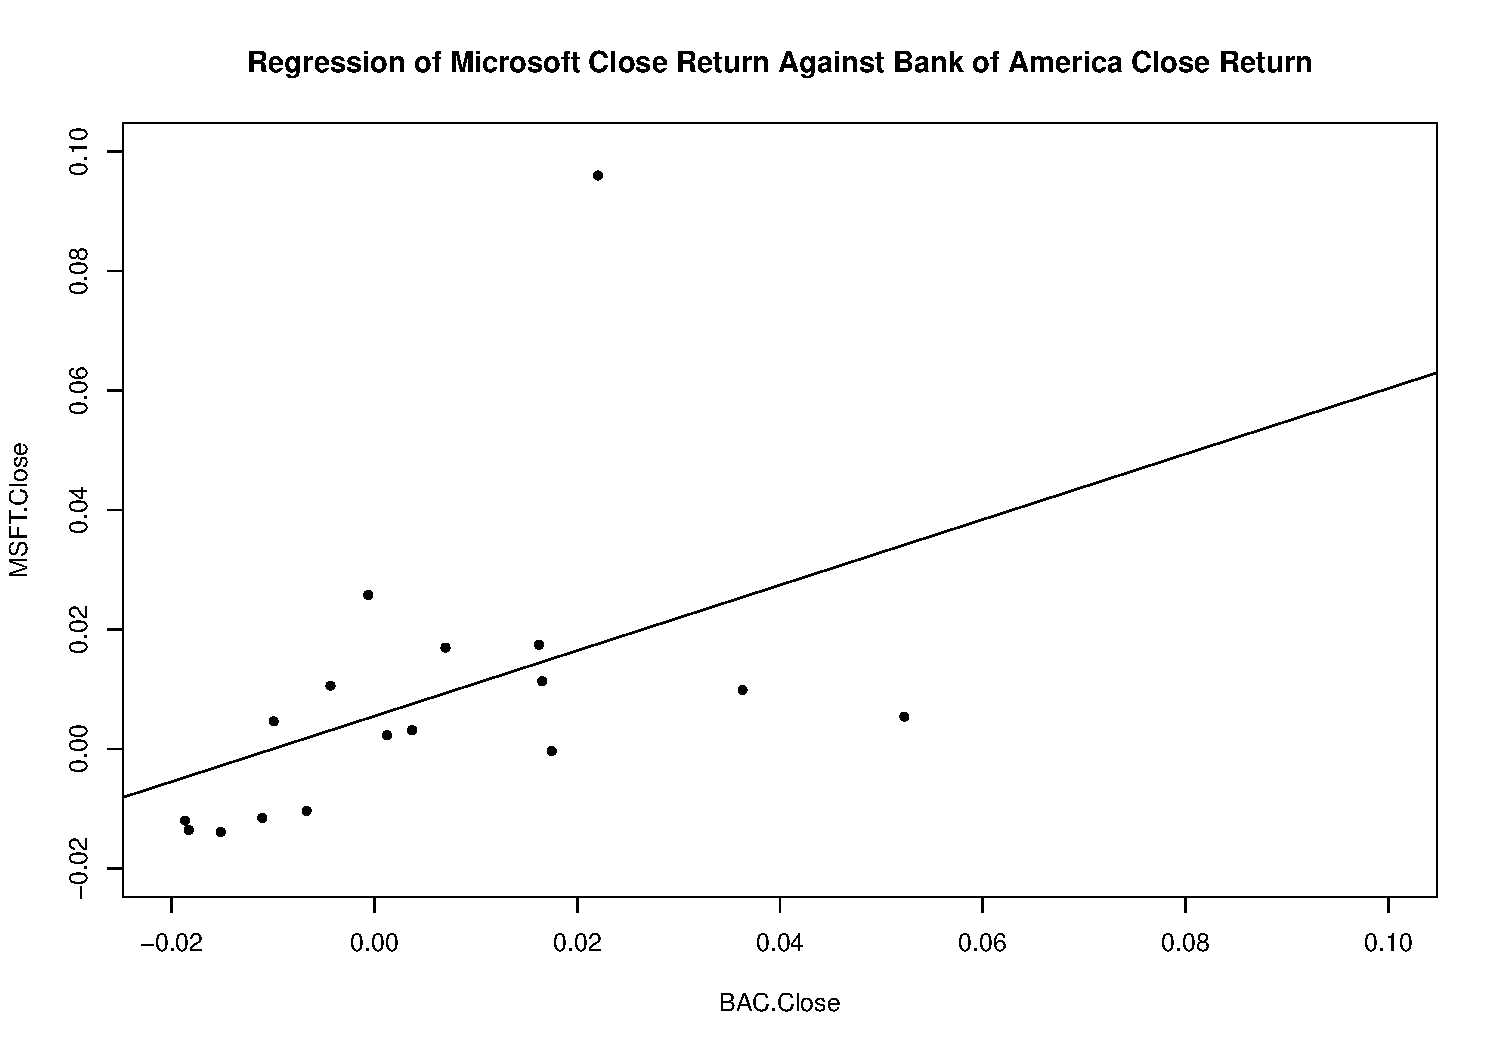
\includegraphics[scale=0.6]{RegRets.pdf}\centering

\raggedright

%----------------------------------------------------------------------------------------

\end{document}